\chapter{Results and Discussion}\label{chap_results}

\section{Model Implementation}

In this chapter the result are presented and discussed. Since the main goal of the work is the packing of the model, the extensive and statistical evaluation of the model is missing.

\subsection{Motor Gestures}

The python implementation of the model allows to easily and quickly explore the sound production model of birds. Using the created objects: syllable, optimizer, birdsongs, paths, and ploter, \ref{Poo}, it is possible to explore and explain how the value parameters impact the output sound (synthetic syllable/birdsong). This is important for a parameters sensitive analysis. 

\begin{figure}[H]
     \centering
     \begin{subfigure}[b]{0.48\textwidth}
         \centering
         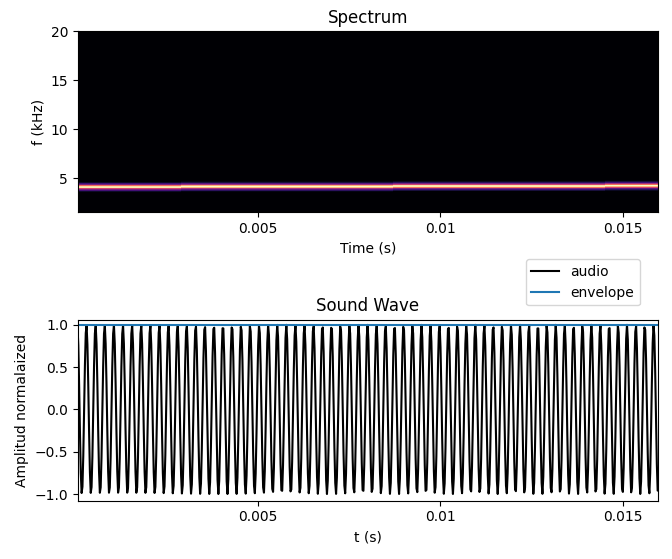
\includegraphics[width=\textwidth]{Images/part_chirp.png}
         \caption{Little part of the input signal, chirp.}
         \label{fig:part_chirp}
     \end{subfigure}
     \hfill
     \begin{subfigure}[b]{0.48\textwidth}
         \centering
         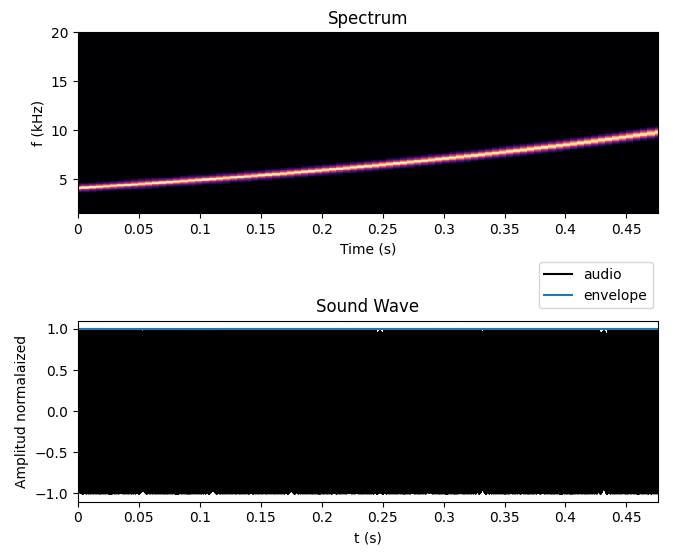
\includegraphics[width=\textwidth]{Images/whole_chirp.png}
         \caption{Whole input signal}
         \label{fig:whole_chirp}
     \end{subfigure}
     \hfill
        \caption{Input chirp signal wave form and spectrogram.}
        \label{fig:chirp}
\end{figure}


As an example consider a pure synthetic case, the external trachea pressure (envelope of the signal function $A=e$, equation \eqref{trache_edos}) is a simple signal (such as a chirp or tone), implying nether audio file or initial coefficient parameters are required. Since this is a simple function, it can be approximated as a quadratic or linear function, then the parameters coefficients can be better understood: the constant coefficient represents a vertical shift for the parameters curves, the linear coefficient gives both vertical and horizontal displacements, and the quadratic coefficient modifies the curvature of the function. In fact, the parameterization of the parameters not only minimizes dimension of the search space, but also provides interpretability for each coefficient. \\

Note that it is possible to define any input signal for the external pressure and explore its impact on the model. Interesting cases are pulses, clicks, tones, or chirp signals, which are easy to experimentally reproduce.\\

First we will study the meaning and impact of the scalar time constant $\gamma$ for the synthetic syllable. For this purpose let us consider some coefficient parameters and three values for $\gamma=1000, 50000,$ and $100000$, Figure \ref{fig:gamma_varying} and the following parameters coefficients $ a = [0.11, 0.05, 0]$ and $ b = [-0.1,1,0] $.

\begin{figure}[H]
     \centering
     \begin{subfigure}[b]{0.48\textwidth}
         \centering
         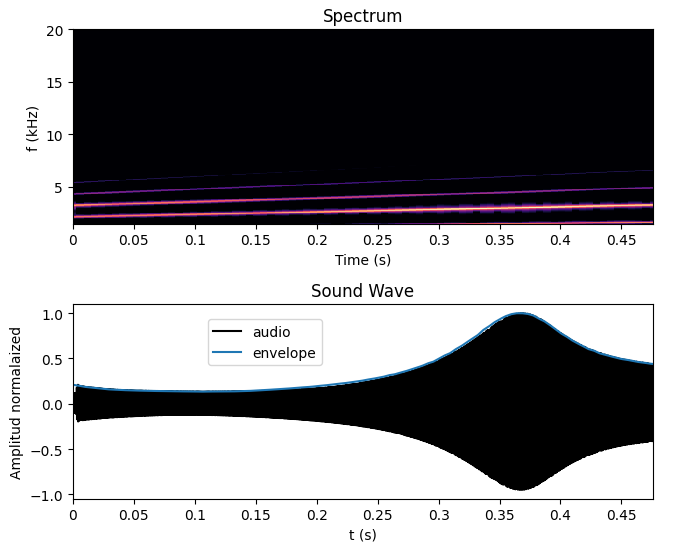
\includegraphics[width=\textwidth, height=5.5cm]{Images/gamma1000.png}
         \caption{$\gamma=1000$}
         \label{fig:gamma1000}
     \end{subfigure}\hfill
     \begin{subfigure}[b]{0.48\textwidth}
         \centering
         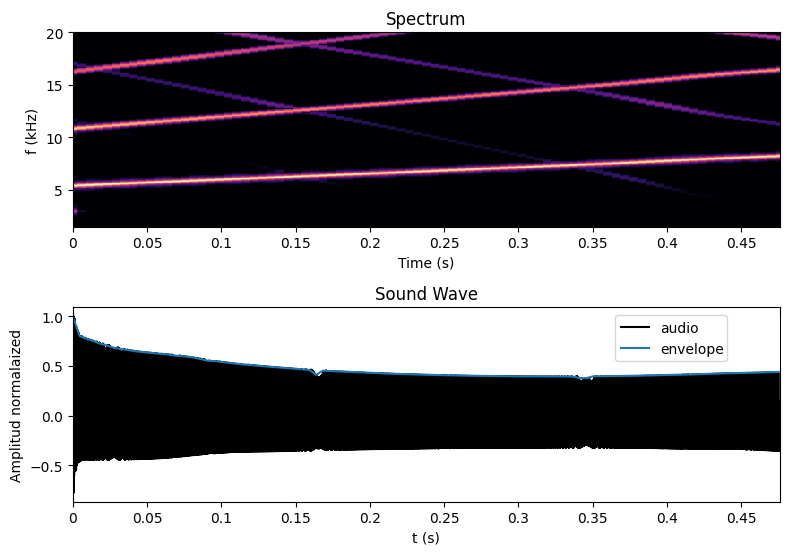
\includegraphics[width=\textwidth, height=5.5cm]{Images/gamma50000.png}
         \caption{$\gamma=50000$}
         \label{fig:gamma50000}
     \end{subfigure}\hfill
     \begin{subfigure}[b]{0.48\textwidth}
         \centering
         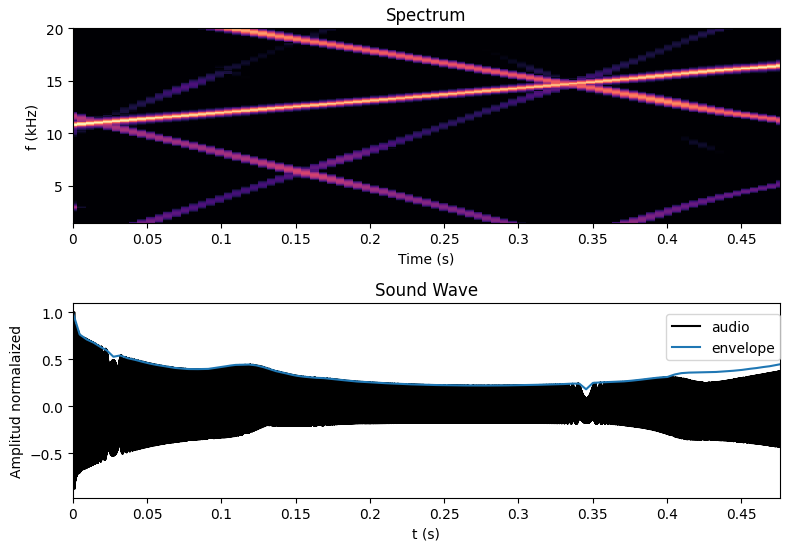
\includegraphics[width=\textwidth, height=5.5cm]{Images/gamma100000.png}
         \caption{$\gamma=100000$ }
         \label{fig:gamma10000}
     \end{subfigure}\hfill
     \begin{subfigure}[b]{0.48\textwidth}
         \centering
         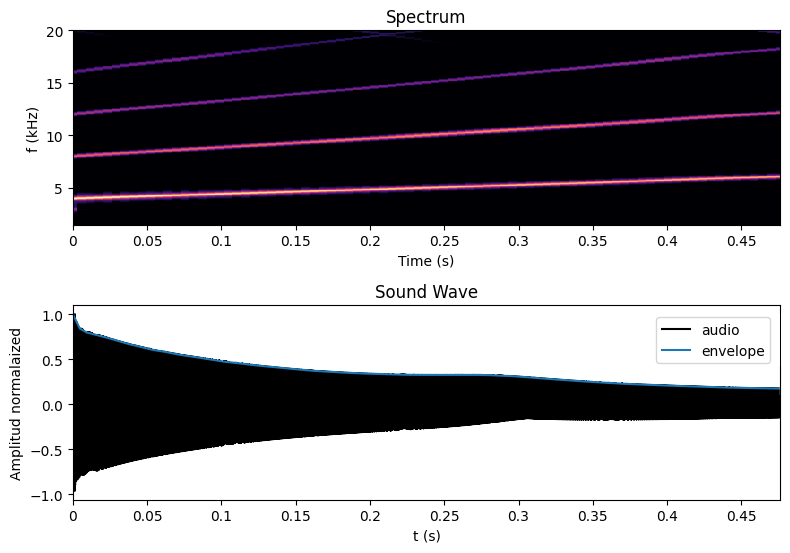
\includegraphics[width=\textwidth, height=5.5cm]{Images/gamma37000.png}
         \caption{$\gamma=37000$ }
         \label{fig:gamma37000}
     \end{subfigure}
        \caption{Spectrogram of output signal varying the time constant scale.}
        \label{fig:gamma_varying}
\end{figure}

When $\gamma$ takes low values the frequency range is small and generates a lower fundamental frequency which may have harmonics (it depends on how far away the sac pressure and labia tension parameters are from the bifurcations, the Hopf bifurcation does not generate harmonics while the Saddle-Nodes do). In contrast, when $\gamma$ takes high values the frequency range increase and many harmonics are present. The optimal values for zonotrichia are those in the middle of the entire range, values between 30000-50000.\\

Now let us explore the impact of the air pressure on the output signal, more so on the fundamental frequency of the synthetic birdsong which is equivalent to exploring different intensities of air pressure from the the bird's lungs entering the syrinx. Let us consider the same coefficient parameters set defined above.

\begin{figure}[H]
     \centering
     \begin{subfigure}[b]{0.48\textwidth}
         \centering
         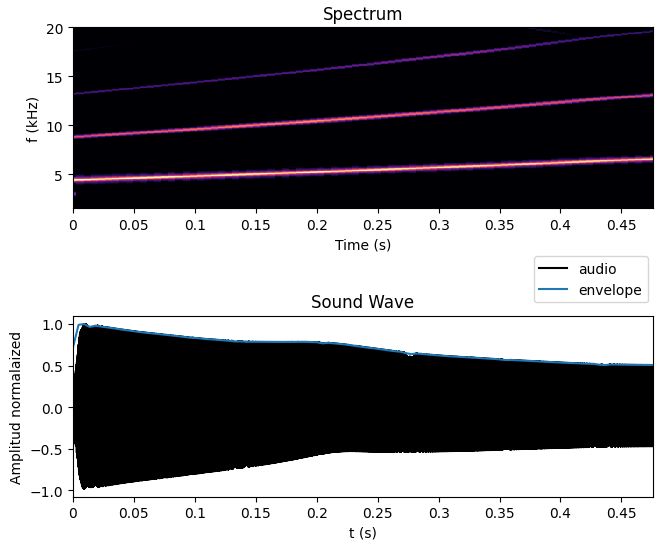
\includegraphics[width=\textwidth, height=7cm]{Images/a001_wave.png}
         \caption{Wave and spectrogram}
         \label{fig:wavea001}
     \end{subfigure}
     \hfill
     \begin{subfigure}[b]{0.48\textwidth}
         \centering
         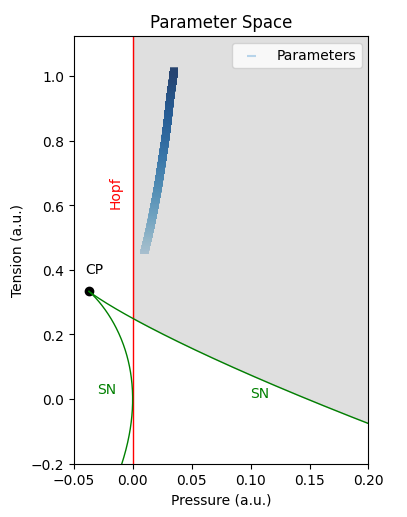
\includegraphics[width=\textwidth, height=7cm]{Images/a001_param.png}
         \caption{Parameters curve an bifurcations}
         \label{fig:parama001}
     \end{subfigure}
     \hfill
        \caption{Low value $a_0=0.01$.}
        \label{fig:a001}
\end{figure}

\begin{figure}[H]
     \centering
     \begin{subfigure}[b]{0.48\textwidth}
         \centering
         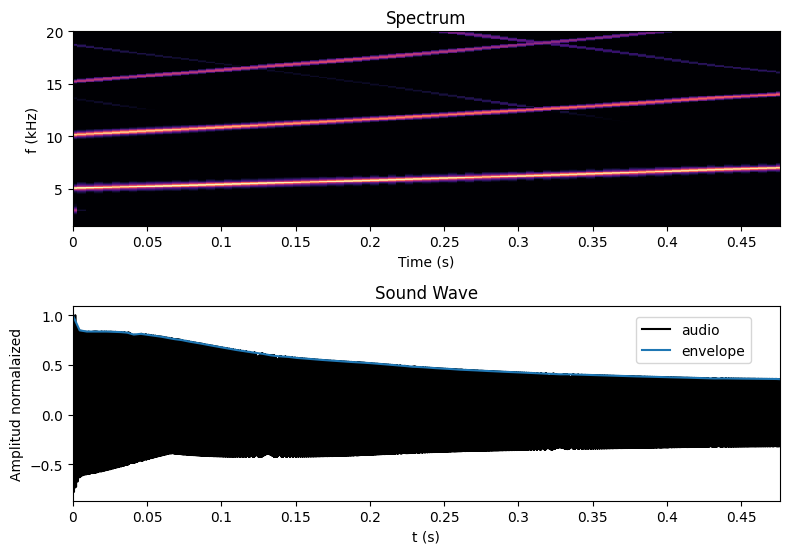
\includegraphics[width=\textwidth, height=7cm]{Images/a011_wave.png}
         \caption{Wave and spectrogram}
         \label{fig:a011}
     \end{subfigure}
     \hfill
     \begin{subfigure}[b]{0.48\textwidth}
         \centering
         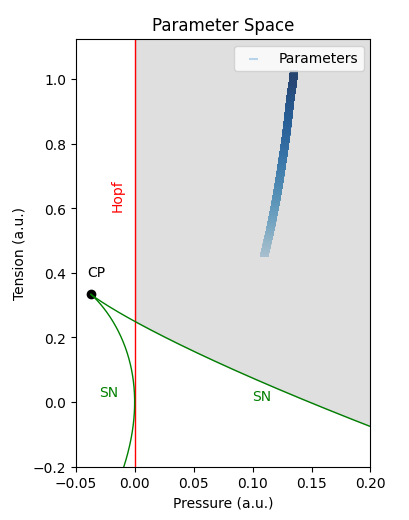
\includegraphics[width=\textwidth, height=7cm]{Images/a011_param.png}
         \caption{Parameters curve an bifurcations}
         \label{fig:a011}
     \end{subfigure}
     \hfill
        \caption{Middle value $a_0=0.11$.}
        \label{fig:a011}
\end{figure}

\begin{figure}[H]
     \centering
     \begin{subfigure}[b]{0.48\textwidth}
         \centering
         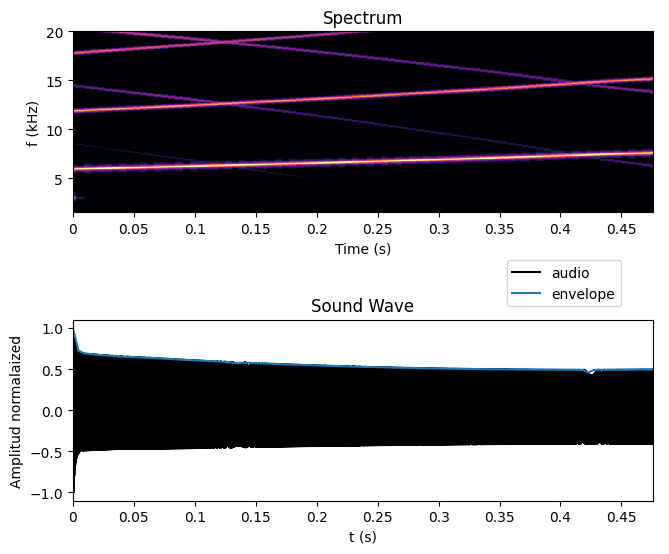
\includegraphics[width=\textwidth, height=7cm]{Images/a125_wave.png}
         \caption{Wave and spectrogram}
         \label{fig:a125wave}
     \end{subfigure}
     \hfill
     \begin{subfigure}[b]{0.48\textwidth}
         \centering
         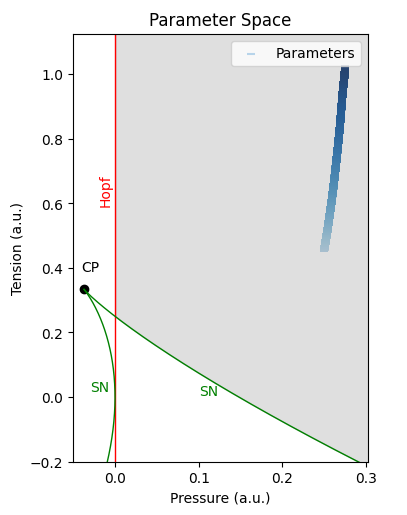
\includegraphics[width=\textwidth, height=7cm]{Images/a125_param.png}
         \caption{Parameters curve an bifurcations}
         \label{fig:a125param}
     \end{subfigure}
     \hfill
        \caption{High value $a_0=1.25$.}
        \label{fig:a125}
\end{figure}

Similarly the parameters space of the labial pressure can be explore. If the audio is less than 10 milliseconds it is defined as a chunck and the labia initial curve is at most a quadratic function defined by its parameters, while if the audio is greater than 10 milliseconds it is defined as a syllable having as initial curve of the labia tension the same fundamental frequency curve but rescaled and dimensionless.

\subsection{Syllable}

The main main bird of study is the Zonotrichia Capensis. They are typical birds in Latin America and specially in Colombia, they are present almost in all the country where we have recorded and published many birdsongs. To study a birdsong, a composition of several syllables or chunck, of any bird it is necessary split the song by syllables and study them one by. Let us study the following Zonotricha birdsong as a syllables and the thrilled part as a chunck, generally this bird has the same form of pitches curves but in the major of cases this pitches has simple shapes.

\begin{figure}[H]
    \centering
    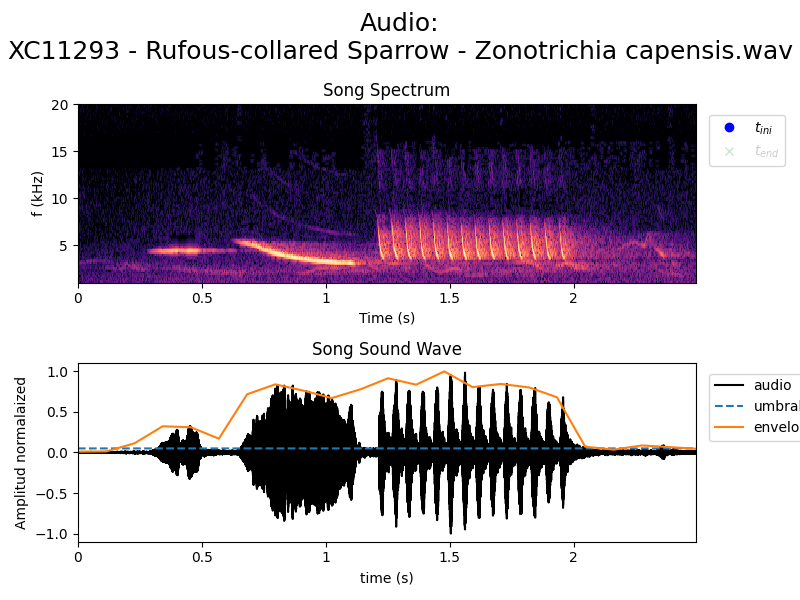
\includegraphics[width=1\linewidth]{Images/Birdsong-XC11293.png}
    \caption{Zonotrichia capensis birdsong sample. It is an audio with noise and three sections of birdsongs: two clear and simple syllables and one series of thrilled syllables. The envelope can be improved with higher Nt object values}
    \label{fig:zonotrichia_all}
\end{figure}


\begin{figure}[H]
    \centering
    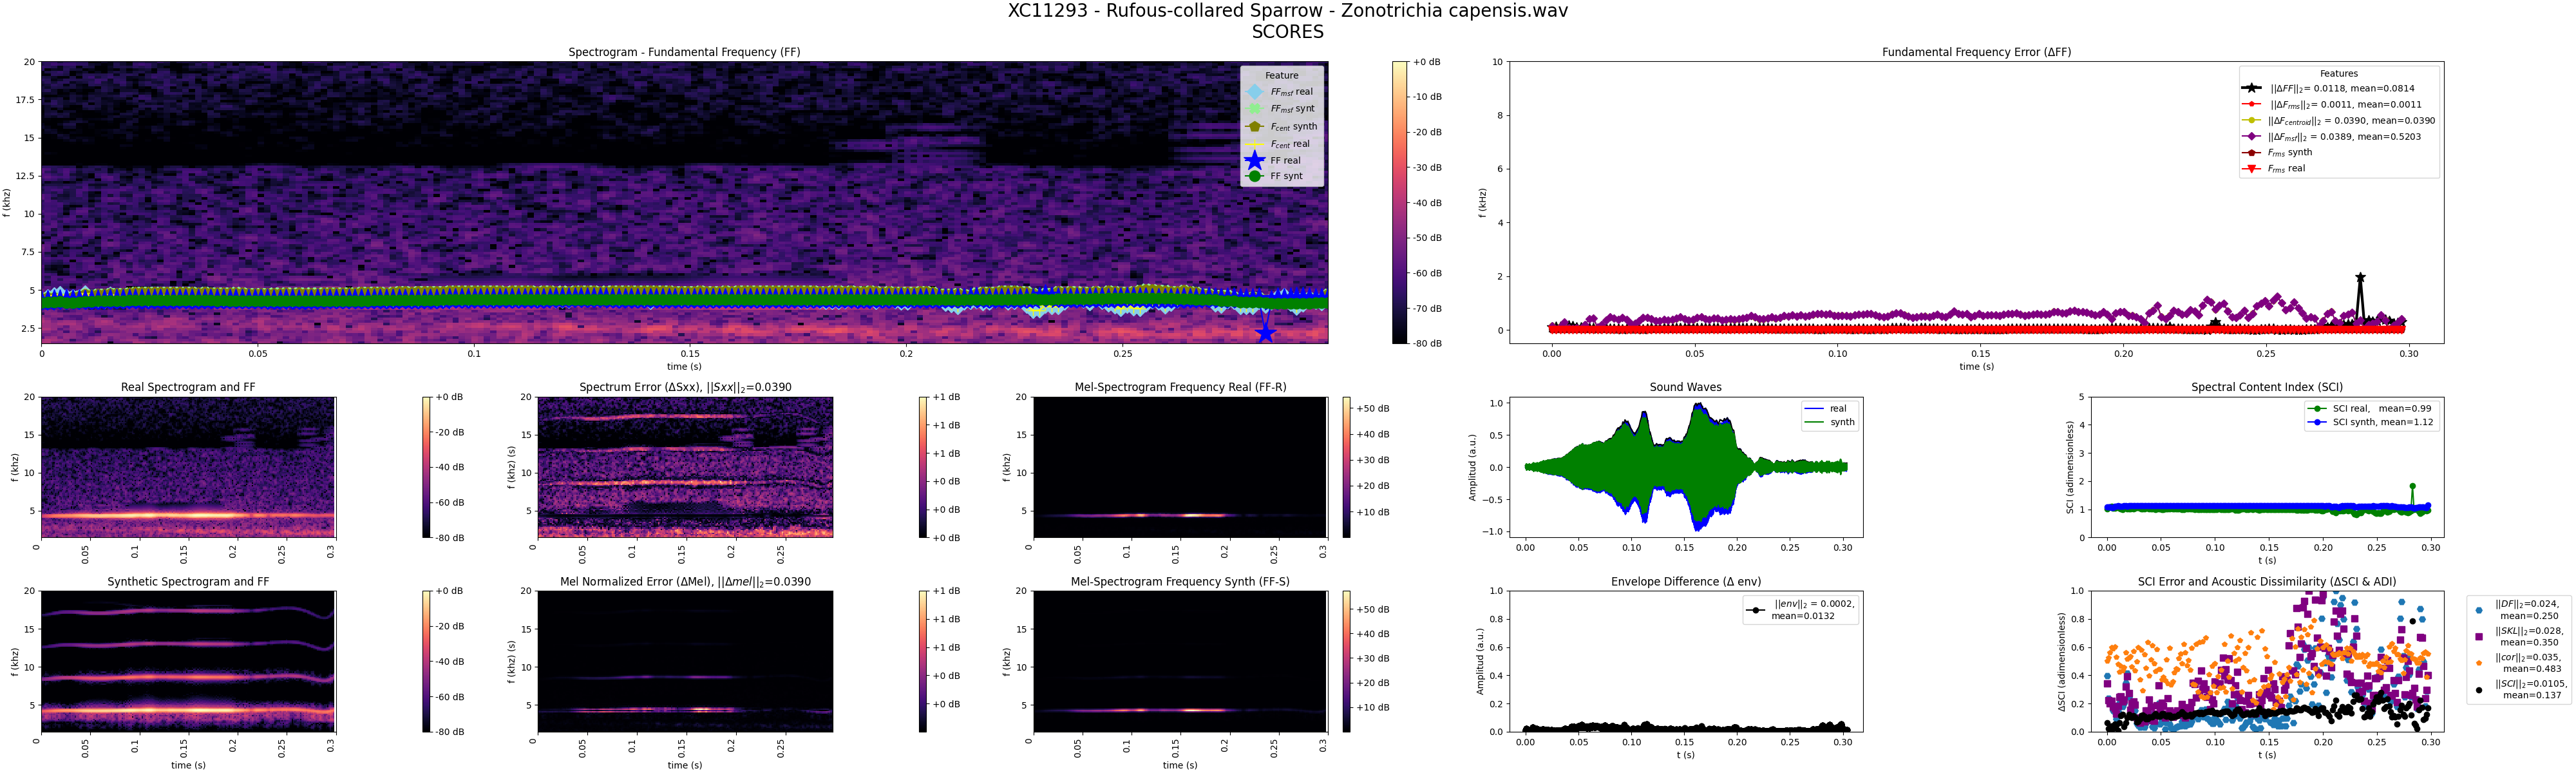
\includegraphics[width=1\linewidth]{Images/ScoresVariables-syllable-XC11293 - Rufous-collared Sparrow - Zonotrichia capensis.wav-1.png}
    \caption{First Zonotrichia capensis syllable. A steady pitch as a pure tone around 5 kHz.}
    \label{fig:zonotrichia_1}
\end{figure}

\begin{figure}[H]
    \centering
    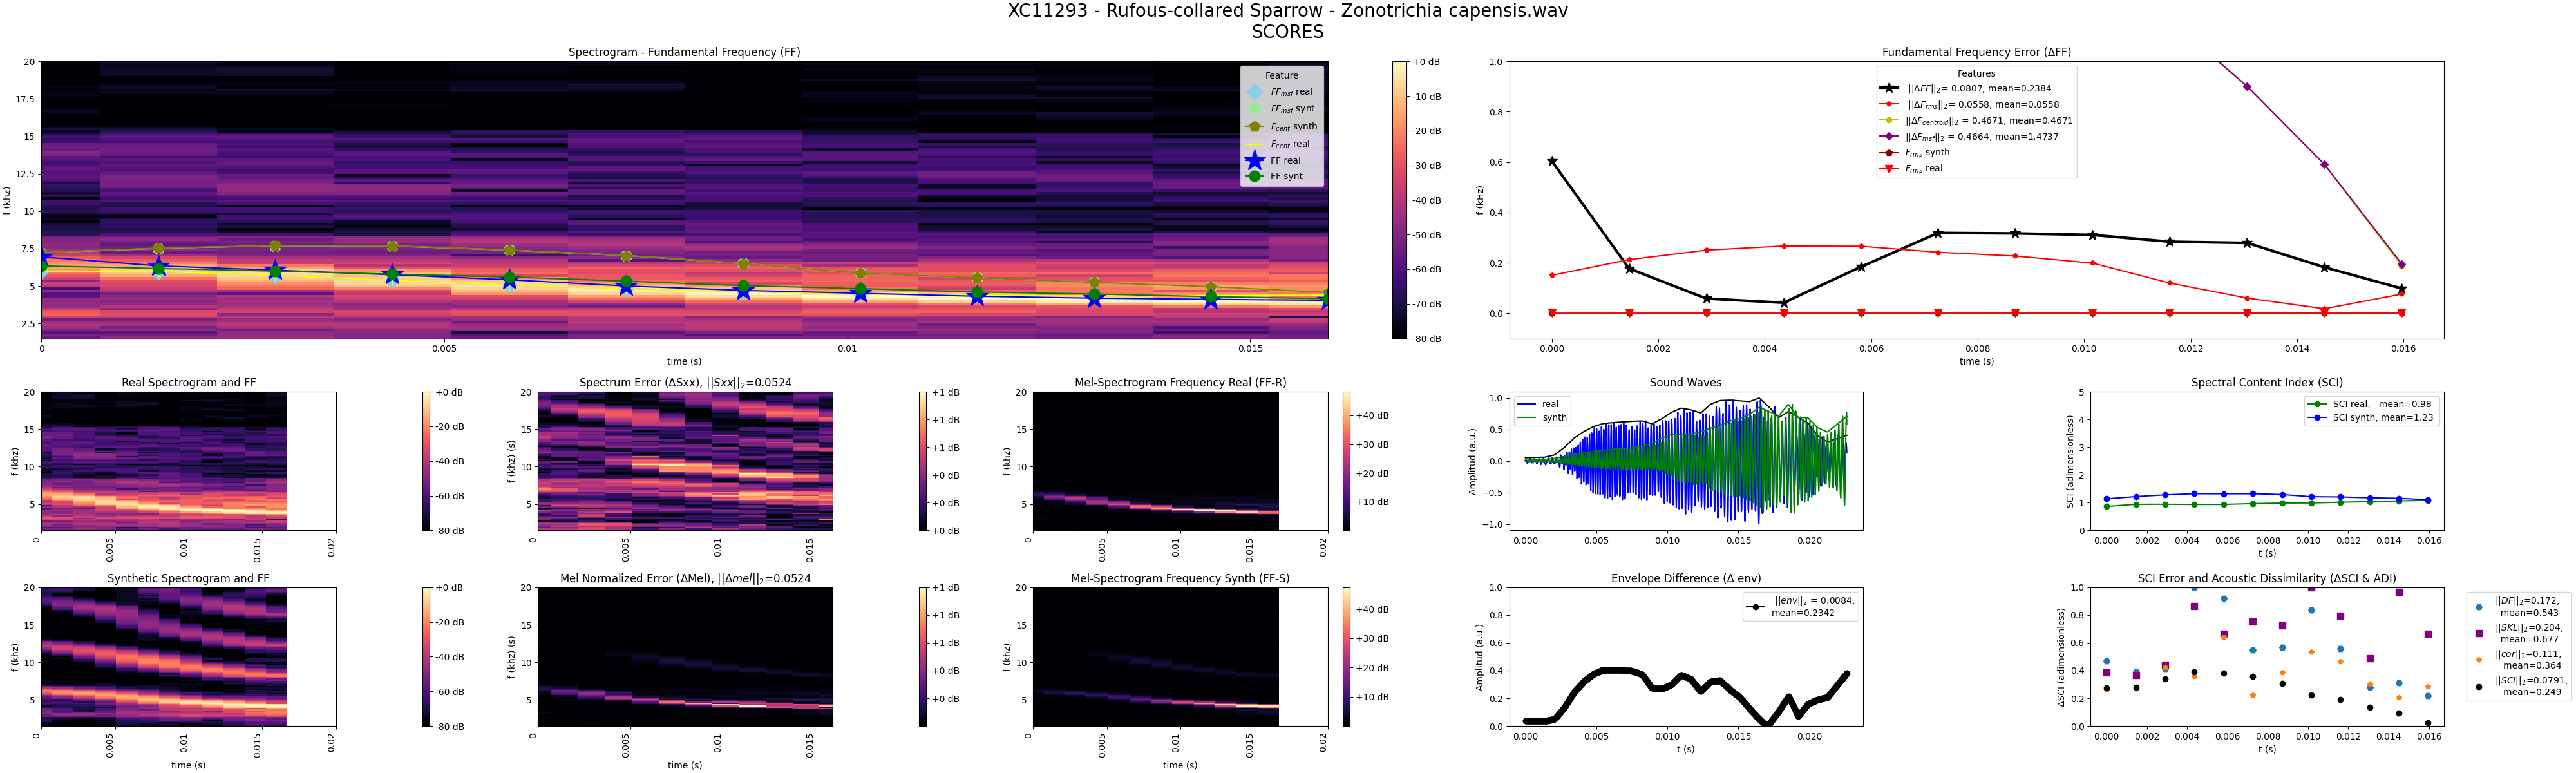
\includegraphics[width=1\linewidth]{Images/ScoresVariables-syllable-XC11293 - Rufous-collared Sparrow - Zonotrichia capensis.wav-0.png}
    \caption{Second Zonotrichia capensis syllable. Decreasing pitch}
    \label{fig:zonotrichia_1}
\end{figure}


\begin{figure}[H]
    \centering
    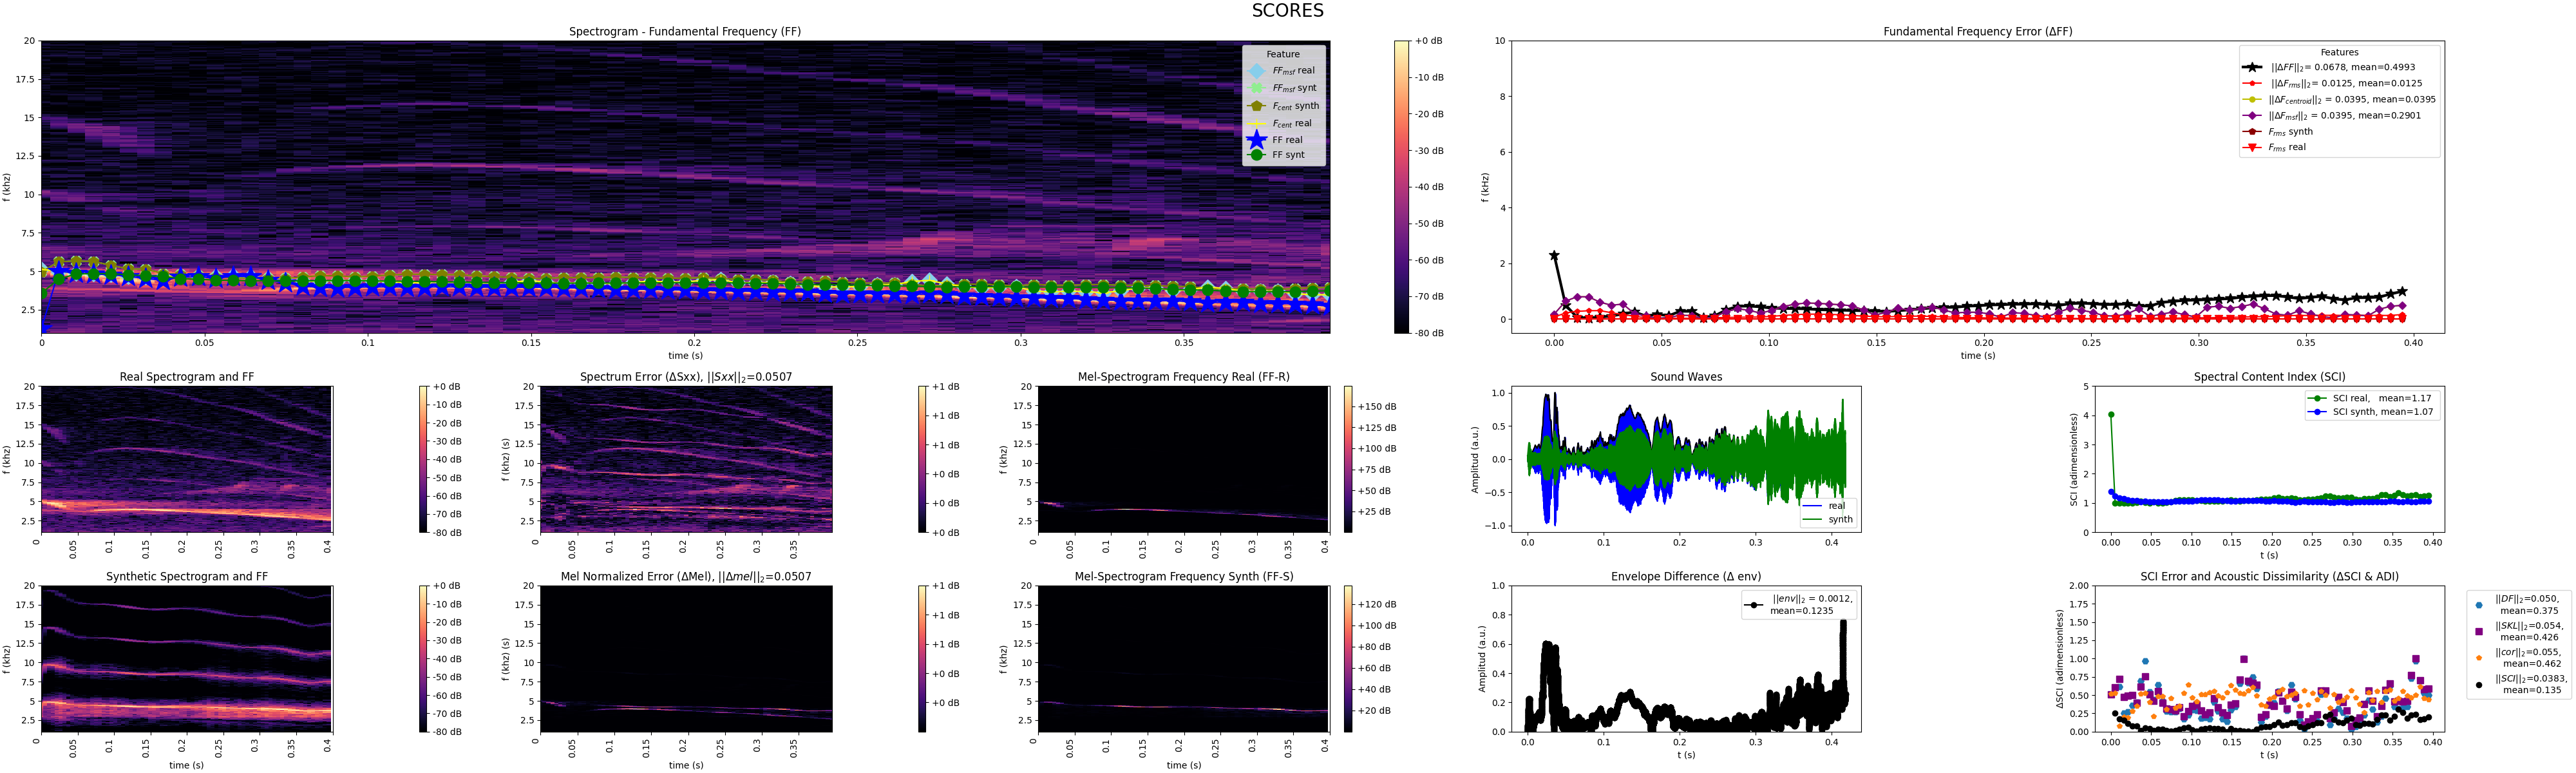
\includegraphics[width=1\linewidth]{Images/ScoresVariables-syllable-4_short_FINCA153_Zonotrichia_capensis_trimed.wav-0.png}
    \caption{Other simple Zonotrichia capensis syllable sample}
    \label{fig:zonotrichia_other}
\end{figure}


\begin{figure}[H]
    \centering
    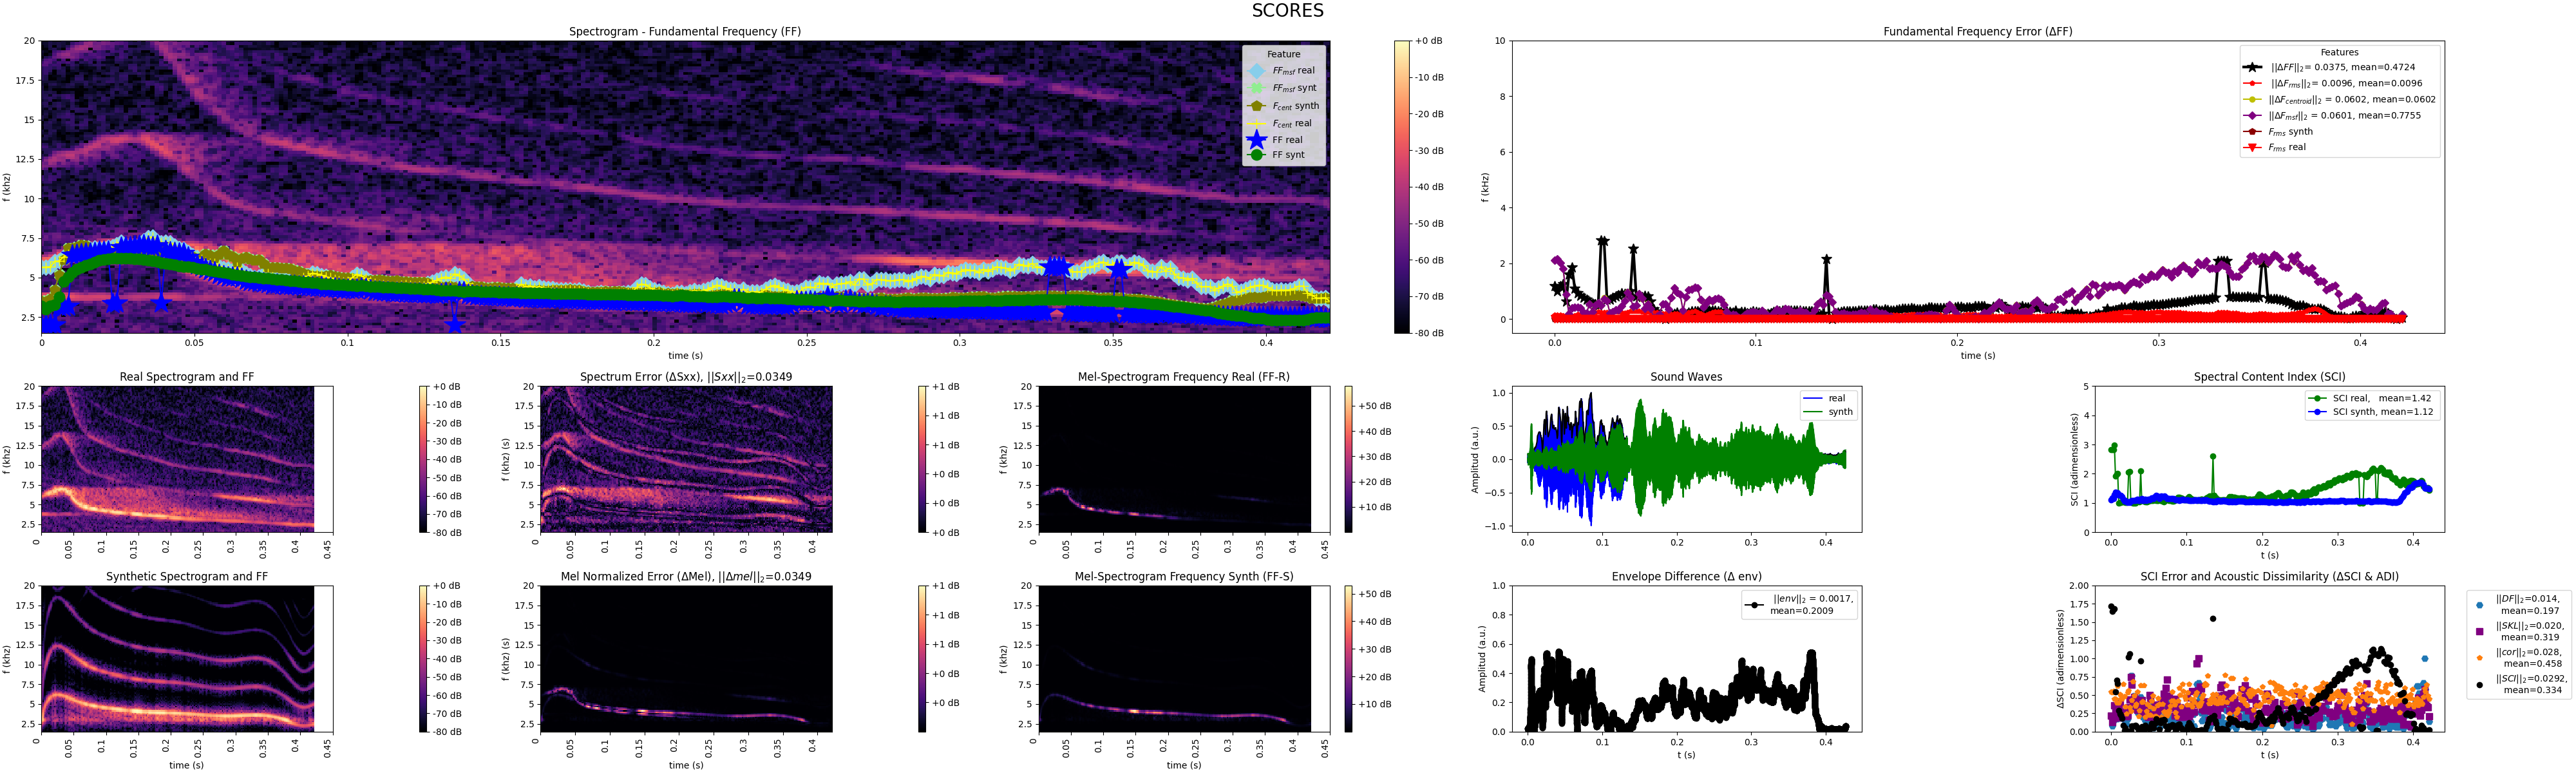
\includegraphics[width=1\linewidth]{Images/ScoresVariables-syllable-2_short_FINCA_H2N_180919-144222_Zonotrichia_capensis.wav-0.png}
    \caption{Complex Zonotrichia capensis syllable sample}
    \label{fig:zonotrichia_complex}
\end{figure}


\subsection{Chunck}

To analyze and generate thrilled birdsong it is necessary to do compute the STFT with small windows length\footnote{the default Fourier window length is 1024 samples but for small time syllables a good window size can be 256 or even 128 (values below can present problems)}, therefore the spectrograms have good frequency resolution but not large time resolution good enough to compute a few pitch points

\begin{figure}[H]
    \centering
    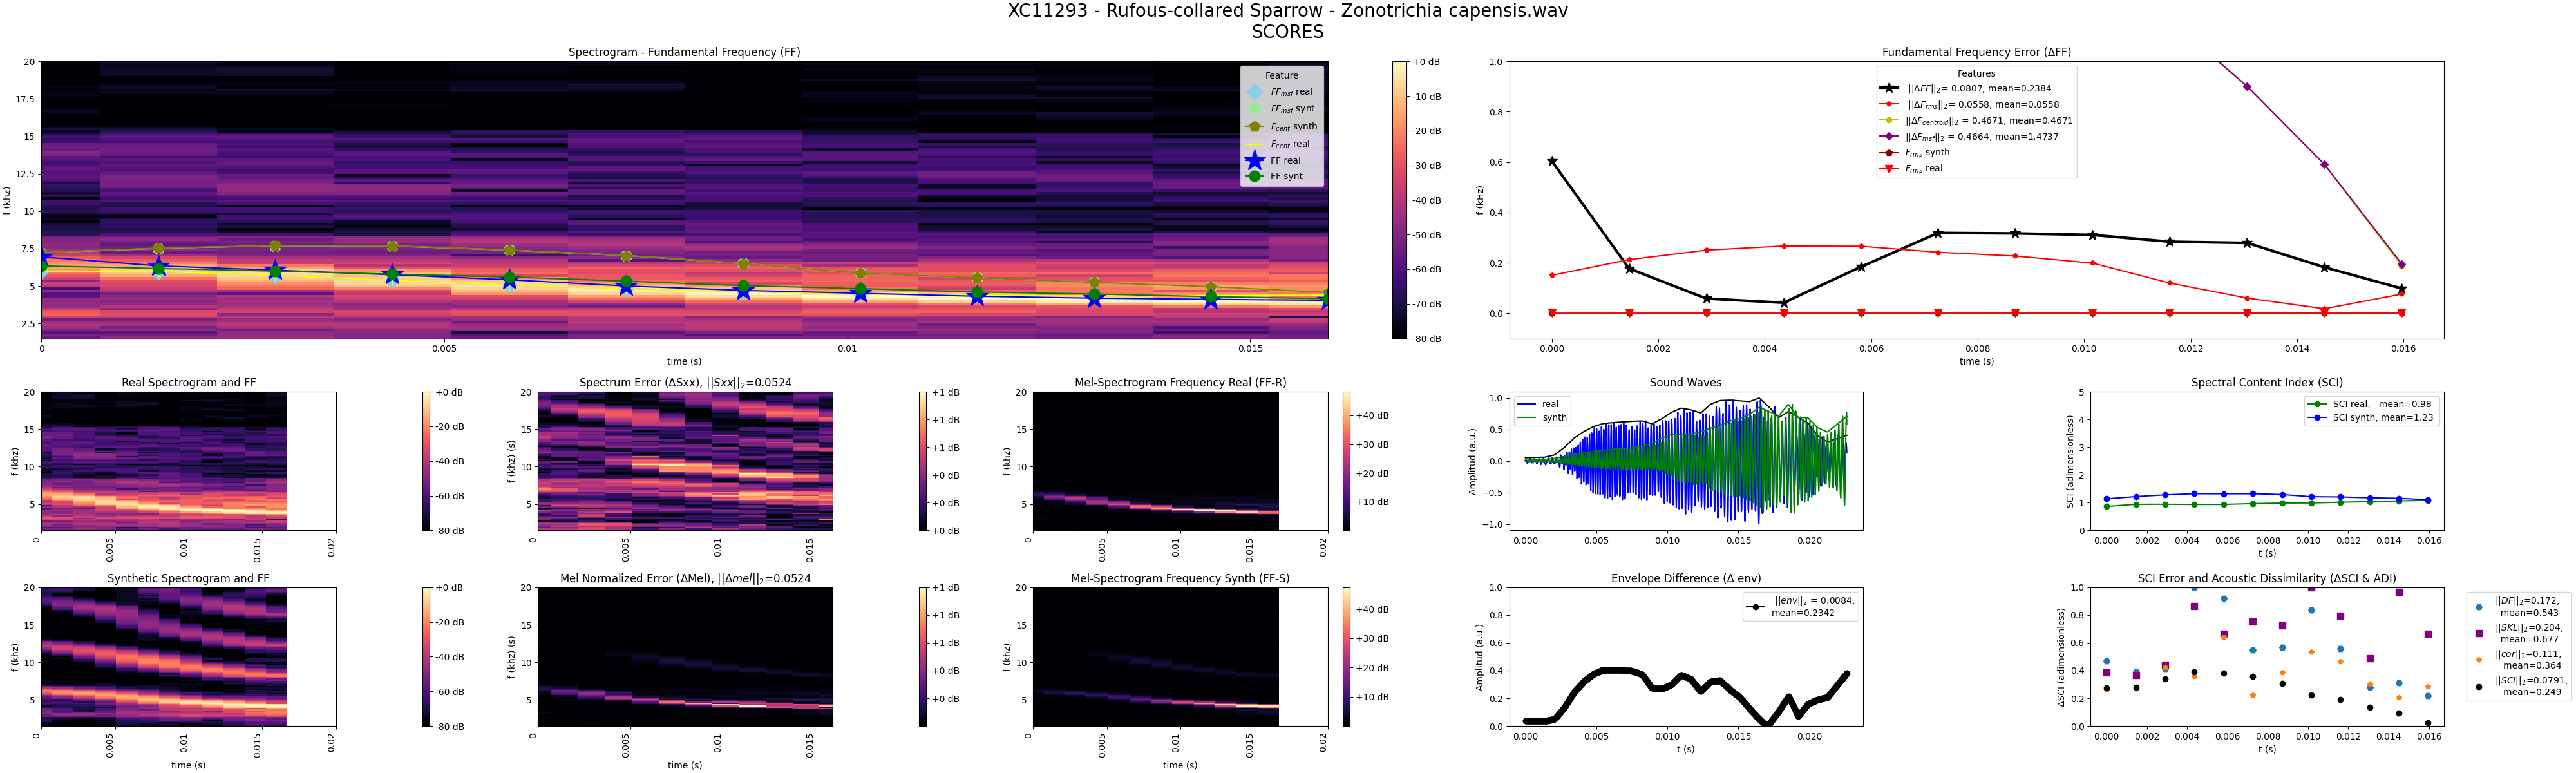
\includegraphics[width=\linewidth]{Images/ScoresVariables-syllable-XC11293 - Rufous-collared Sparrow - Zonotrichia capensis.wav-0.png}
    \caption{Third and small syllable of the Zonotrichia capensis sample. It is part of a series of thrilled syllables whit the same pitch shape and steady tendency}
    \label{fig:}
\end{figure}

While the real spectrogram does not have strong harmonics, but has noise, the synthetic birdsong have many harmonics. This occurs because the noise is interpreted as harmonic content by the spectral content and acoustic dissimilarity indexes. The result is very good in pitch and in SCI with small errors in both quantities, other spectral variables also presented good results ($f_{rms} $ and spectral centroid).

\subsection{Birdsong}

Computing syllable by syllable is very time consuming, since to get a good result it is necessary to adjust the pitch threshold and sometimes the samples length of the Fourier window. For this reason, the birdsong package also provides a possible synthetic birdsong generation by selecting some interval points and then using them in a  birdsong method to find the optimal set of  parameters values to each syllable\footnote{the optimal value of $\gamma$ is the mean of all the optimal values found each syllable considering a well defined initial parameters set values, such that generates oscillations and are not too close to bifurcations}


\begin{figure}[H]
    \centering
    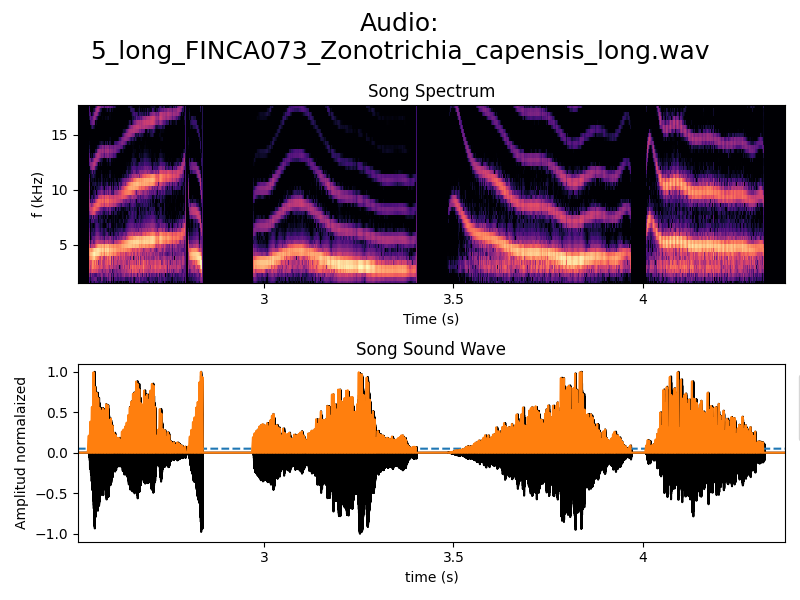
\includegraphics[width=\linewidth]{Images/Figure 23.png}
    \caption{Real Zonotrichia birdsong .}
    \label{fig:birdsong_real}
\end{figure}

\begin{figure}[H]
    \centering
    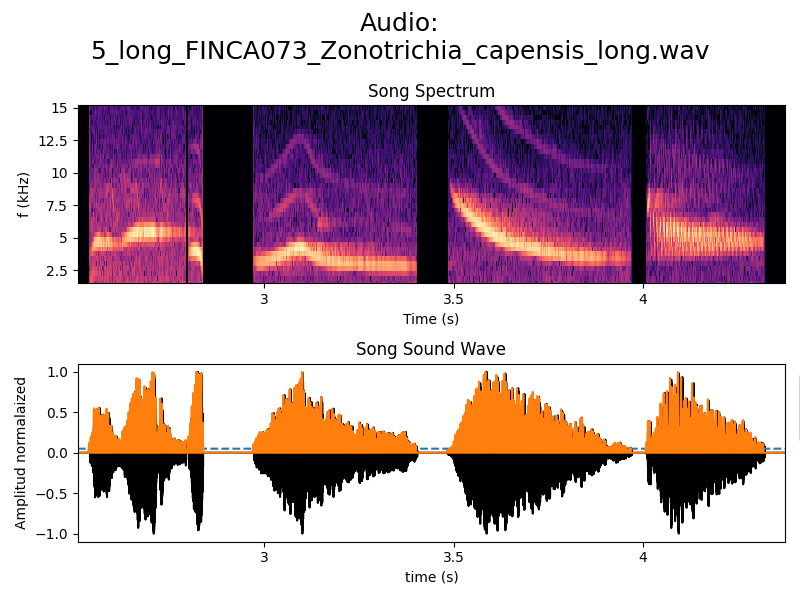
\includegraphics[width=\linewidth]{Images/Figure 26.png}
    \caption{Synthetic Zonotrichia birdsong .}
    \label{fig:birdsong_real}
\end{figure}




\begin{figure}[H]
    \centering
    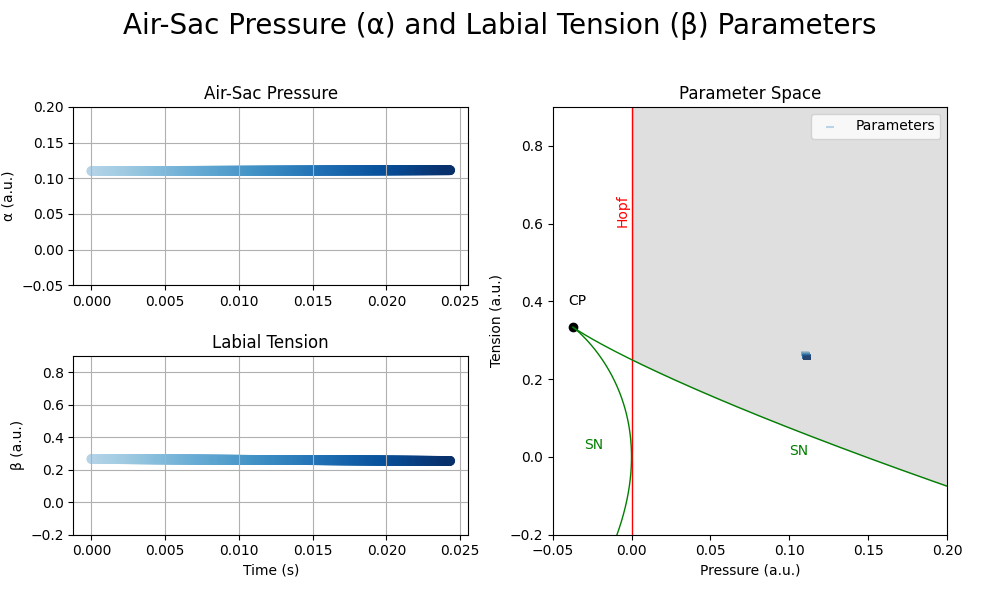
\includegraphics[width=\linewidth]{Images/Results/MotorGesturesParameters-chunck-synth-1-0.png}
    \caption{Parameters space and curve of the parameters}
    \label{fig:result_alphabeta}
\end{figure}

\begin{figure}[H]
    \centering
    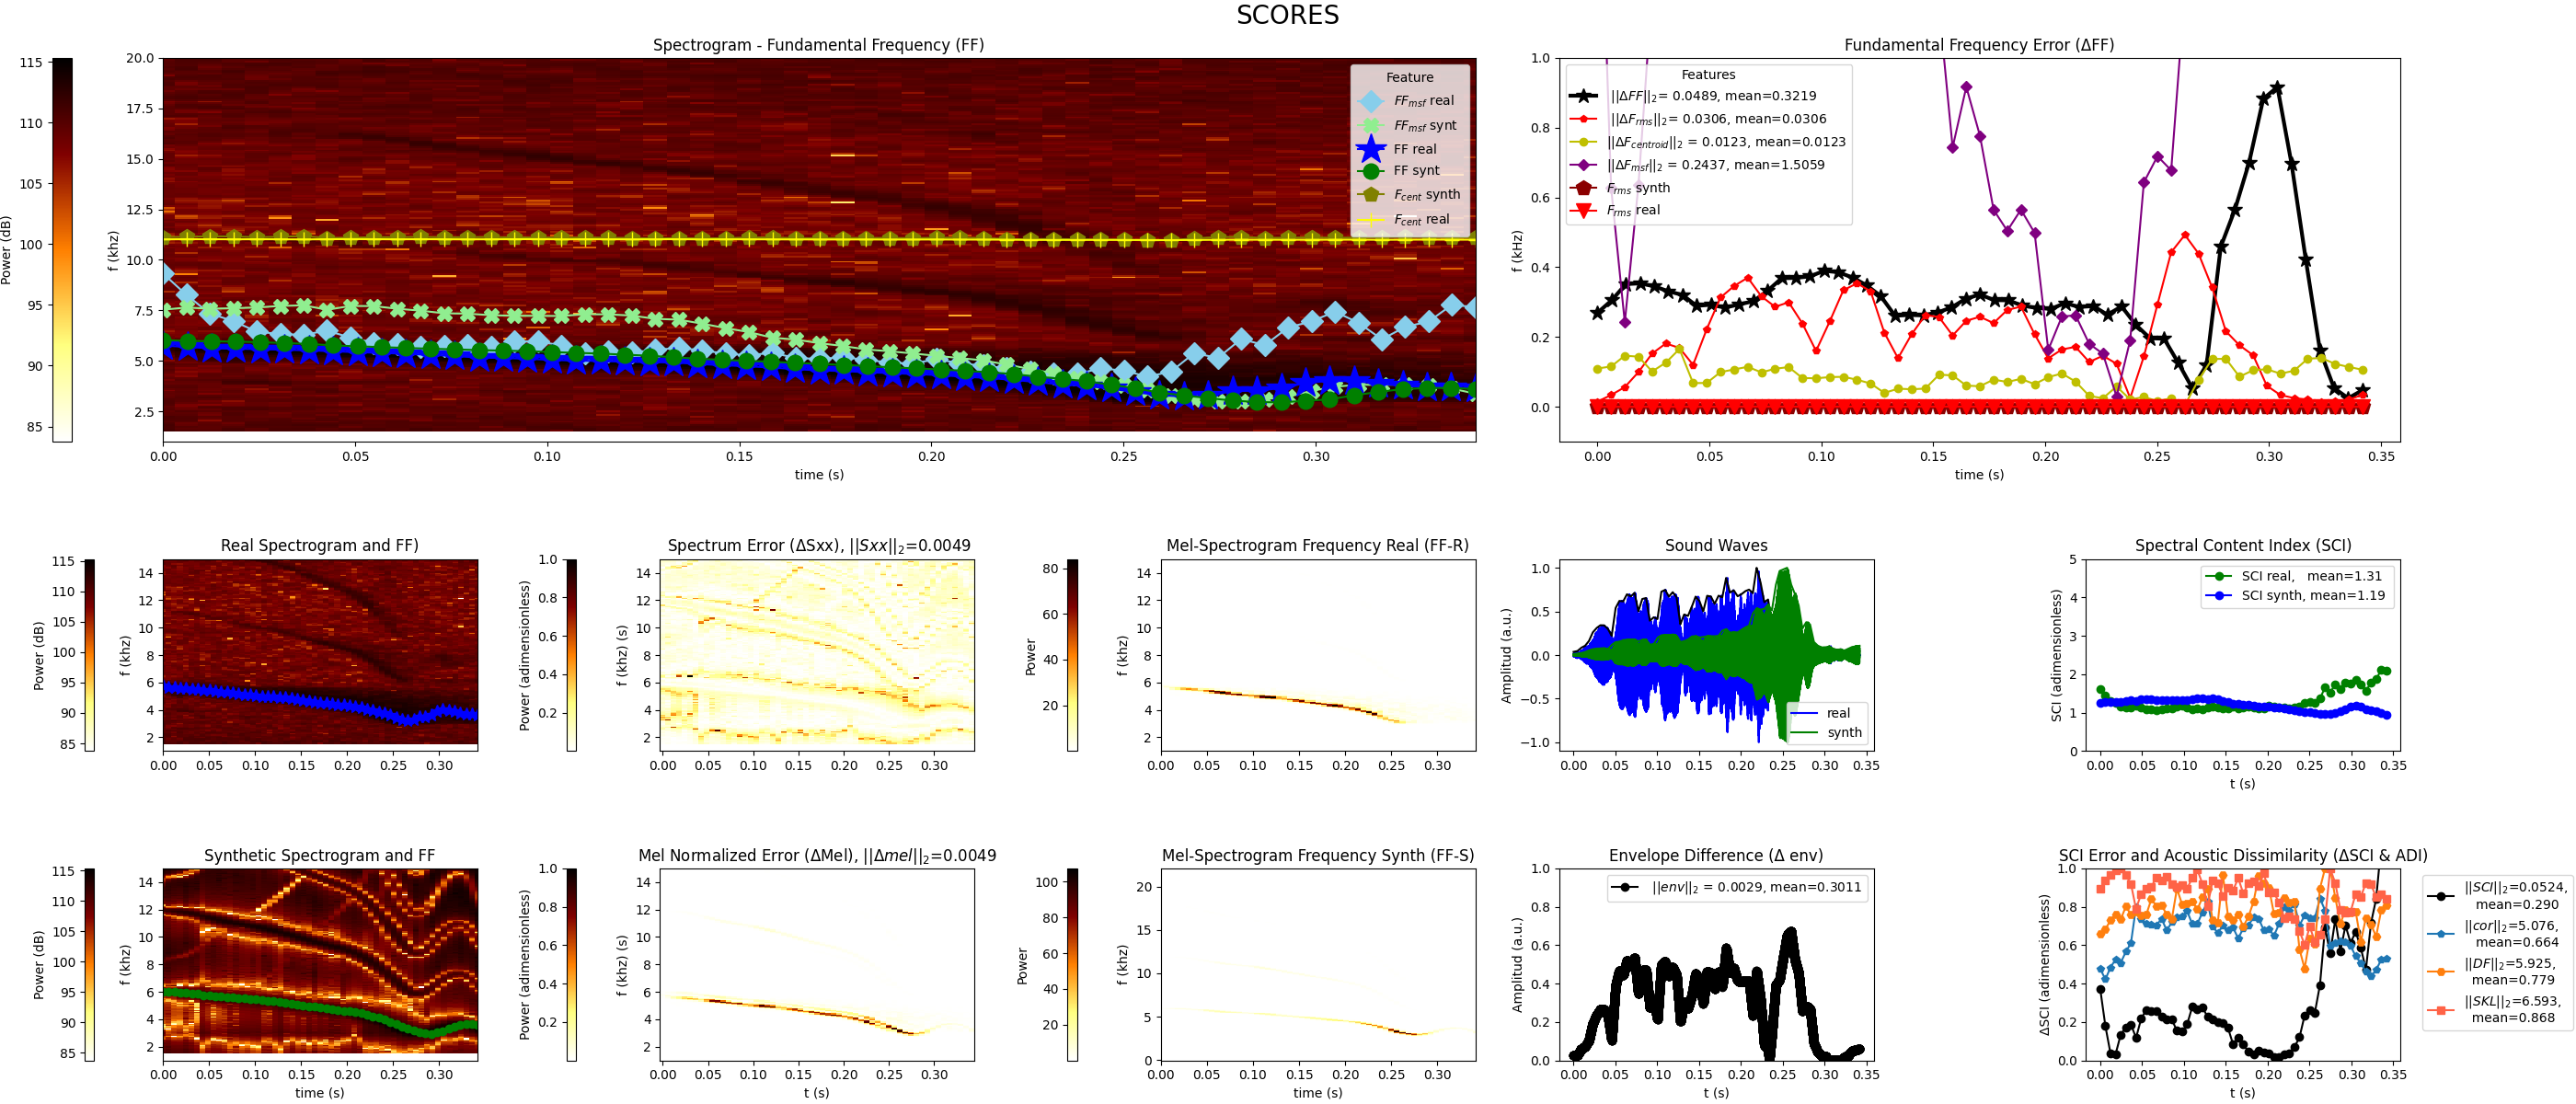
\includegraphics[width=1.\linewidth]{Images/Results/ScoresVariables-syllable-1-1.png}
    \caption{Synthetic and real syllables comparison}
    \label{fig:result}
\end{figure}








\section{Evaluation}

\subsection{Consistency}

\begin{enumerate}
    \item Generate a synthetic syllable with random parameters.
    
    \begin{figure}[H]
    \centering
    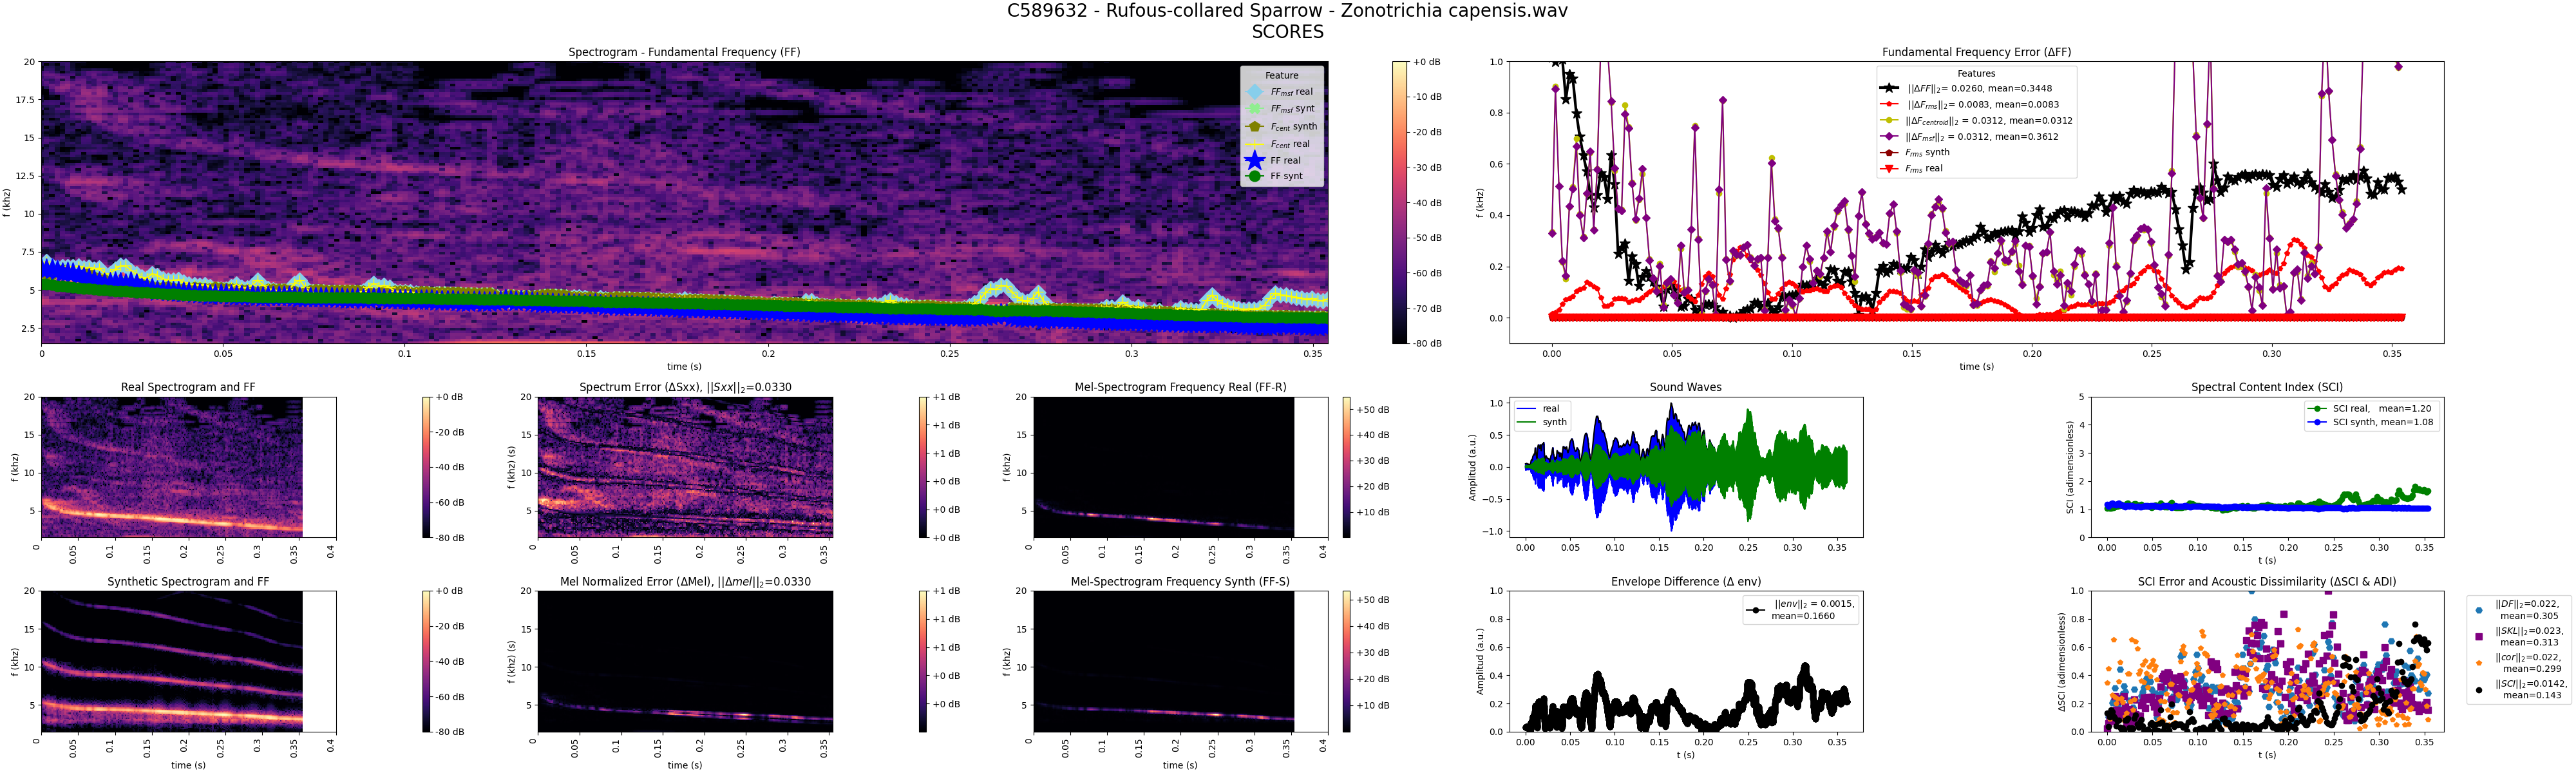
\includegraphics[width=\linewidth]{Images/1.png}
    \caption{First optimal solution}
    \label{fig:first_optimal}
    \end{figure}
    
    \item Solve the optimization problem for the generated syllable.
    
    \begin{figure}[H]
    \centering
    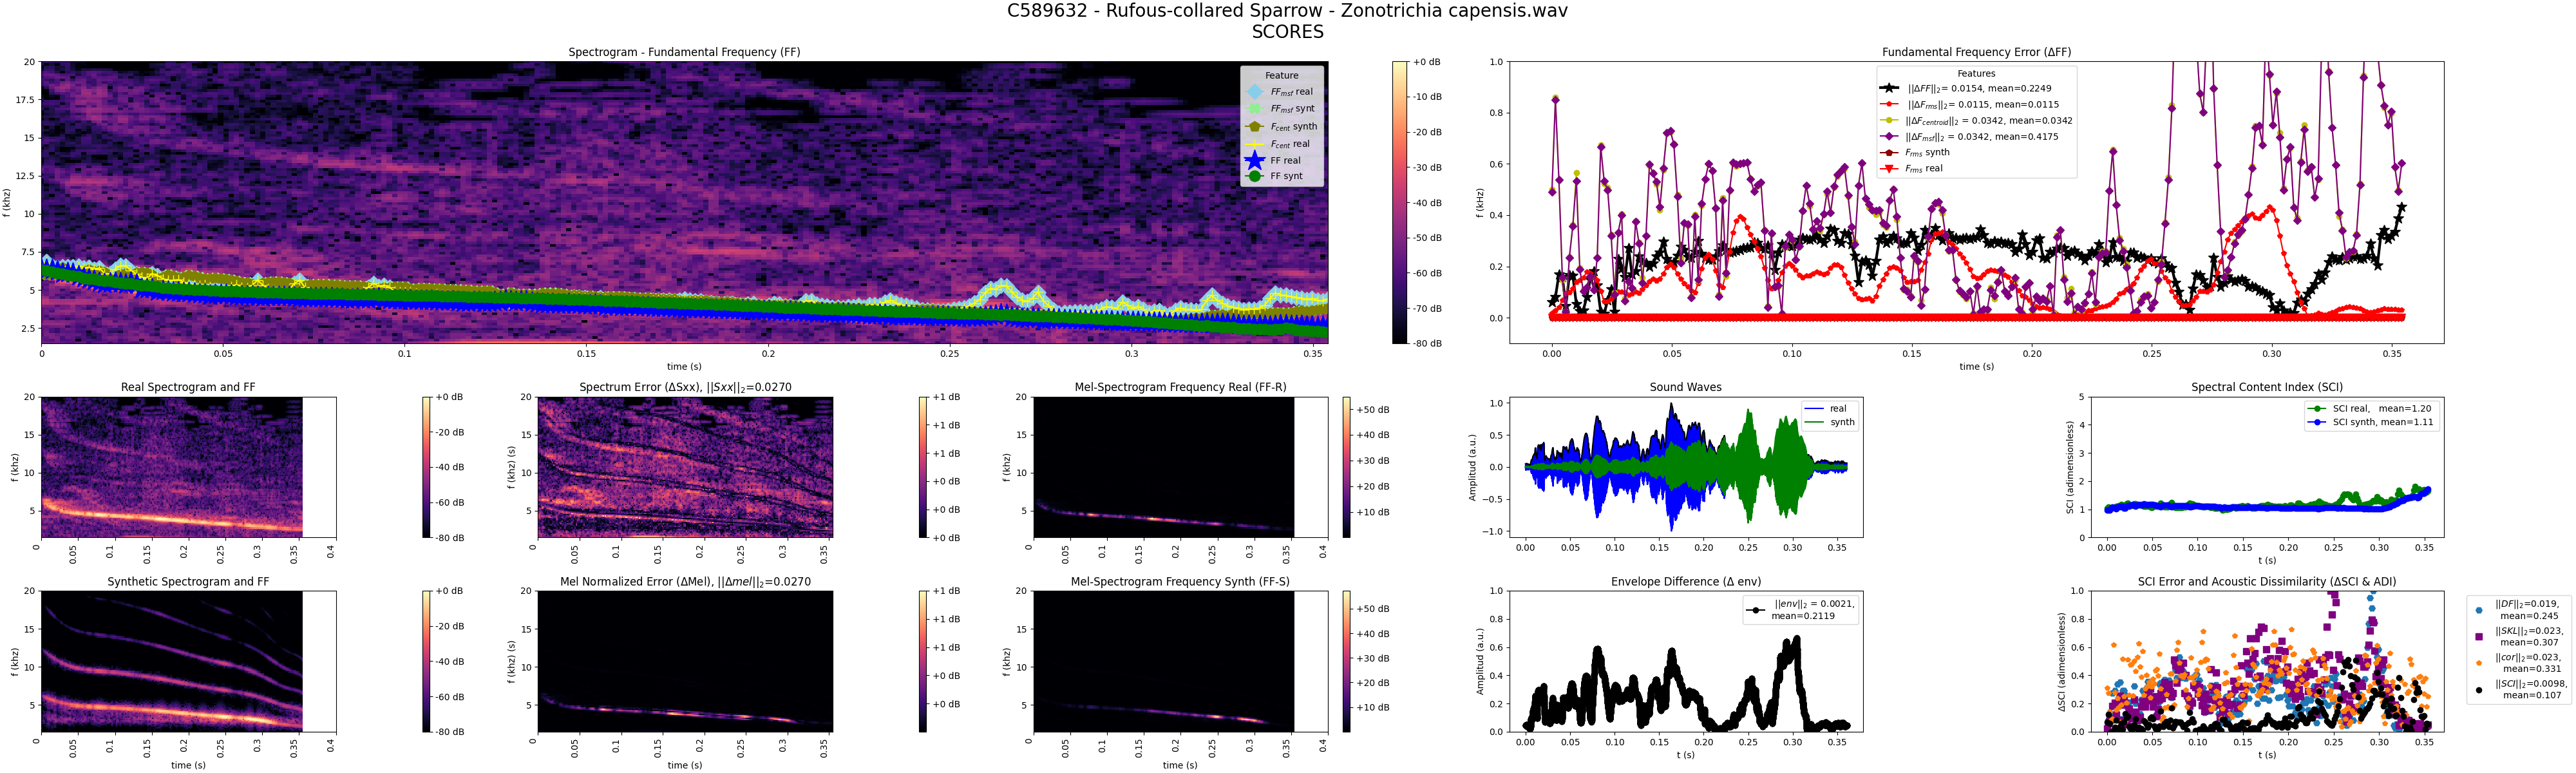
\includegraphics[width=\linewidth]{Images/2.png}
    \caption{Optimal solution of the previous optimal solution}
    \label{fig:second_optimal}
    \end{figure}
    
    
    \item Compare features
    
    Synthetic syllables generated by the model solution twice
    
    \begin{figure}[H]
    \centering
    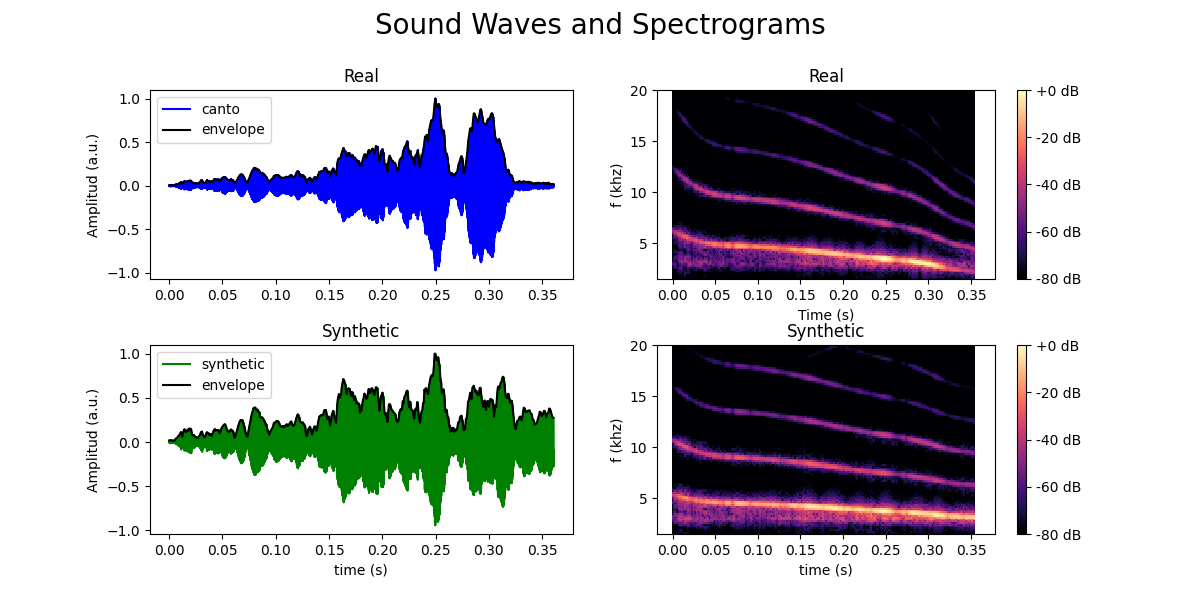
\includegraphics[width=\linewidth]{Images/3.png}
    \caption{Comparison of the optimal solution (top) for the real birdsong, and the optimal solution for the synthetic syllable (bottom).}
    \label{fig:comparison_synth}
    \end{figure}
    
\end{enumerate}

\subsection{Uniqueness}

Since the parameters space have at most 7 dimension, the optimization problem has not a single optimal and different parameters sets may generate the same syllable. The proposed method reach a local minima by solving the optimization subproblems. 


\subsection{Generalization}

For the Zonotricha capensis the birdsong package works efficiently and generated good qualitative and quantitative results, comparable birdsongs. To testing the model generalization other species are used, they are listed in order of pitch complexity from the easiest one.


\begin{enumerate}
    \item Tapaculos (Rhinocryptidae): pitches are elementary functions that can be approximate as linear or quadratic functions 
    
    \begin{figure}[H]
    \centering
    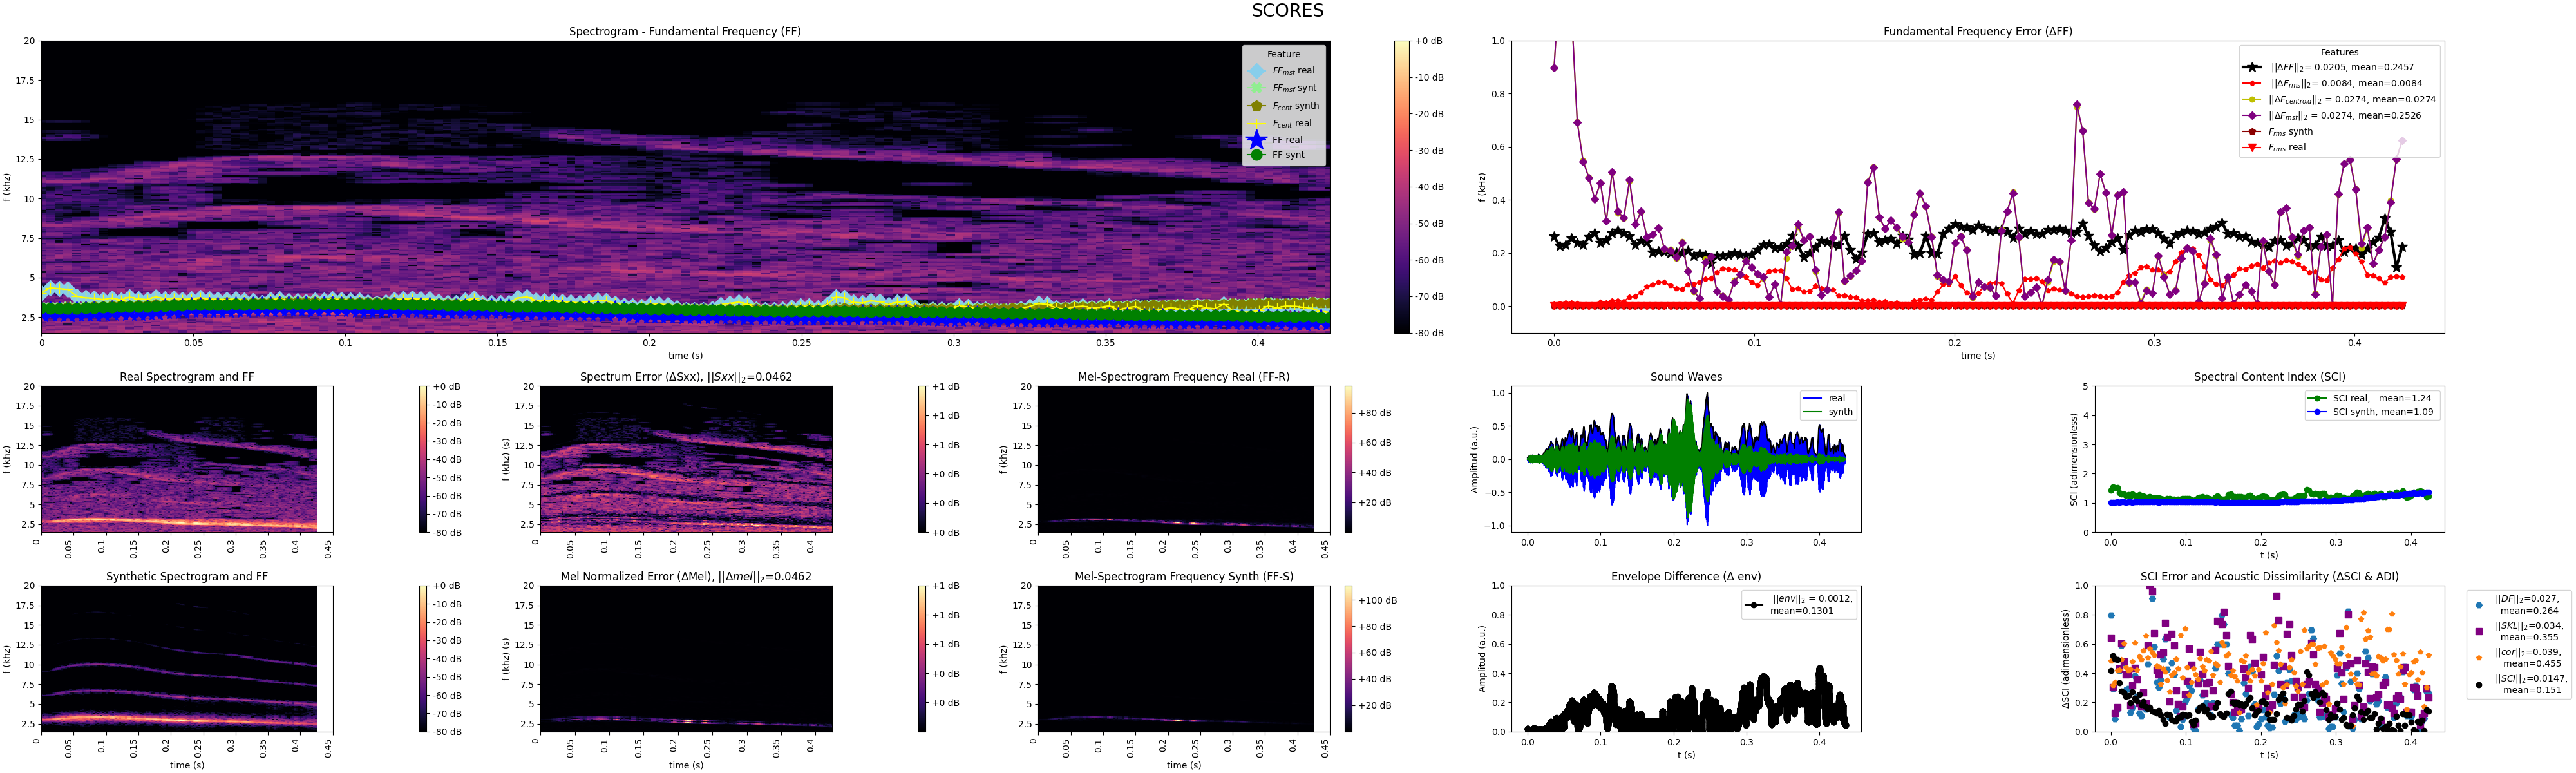
\includegraphics[width=1\linewidth]{Images/ScoresVariables-syllable-XC104508 - Ocellated Tapaculo - Acropternis orthonyx.wav-0.png}
    \caption{Simple Tapaculos syllable sample}
    \label{fig:tapaculos}
    \end{figure}
    
    
    \item Euphonia laniirostris 
    \begin{figure}[H]
    \centering
    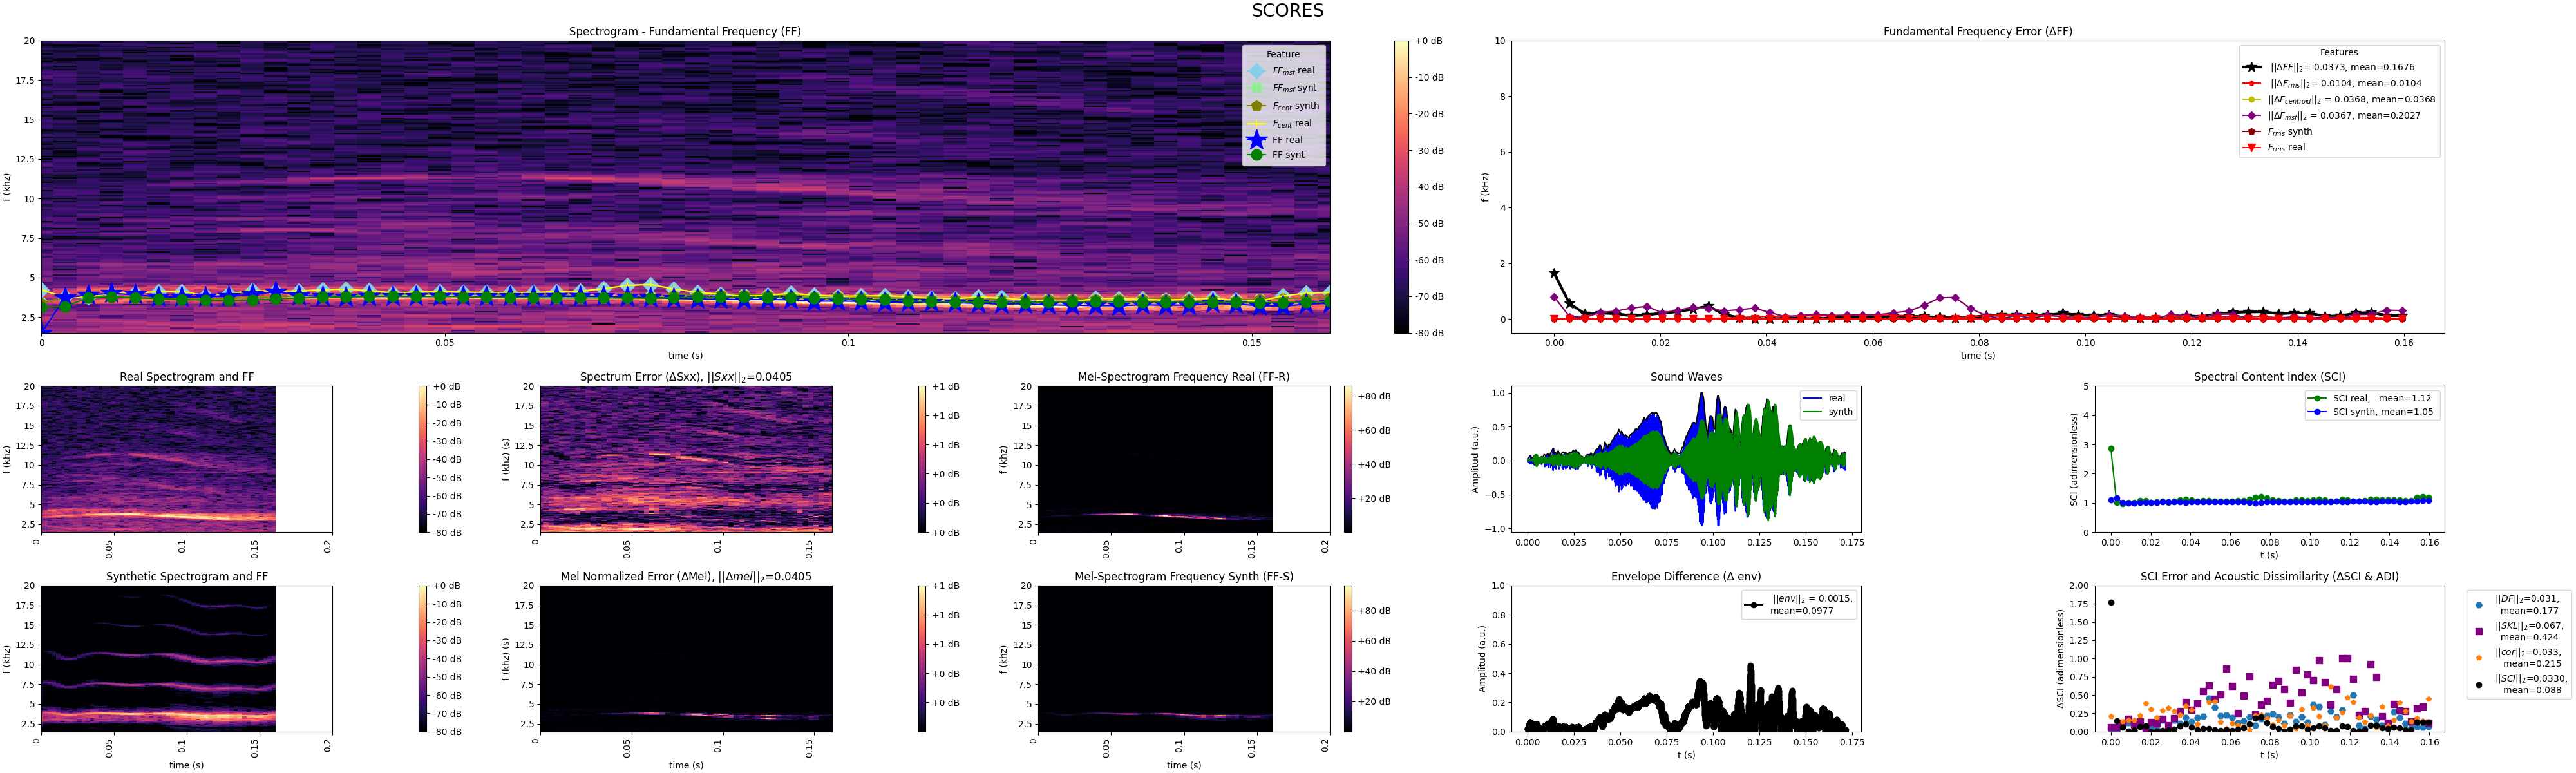
\includegraphics[width=1\linewidth]{Images/ScoresVariables-syllable-C527995 - Thick-billed Euphonia - Euphonia laniirostris.wav-0.png}
    \caption{Simple Euphonia laniirostris syllable sample}
    \label{fig:tapaculos}
    \end{figure}
    
    \item Mimus gilvus
    \begin{figure}[H]
    \centering
    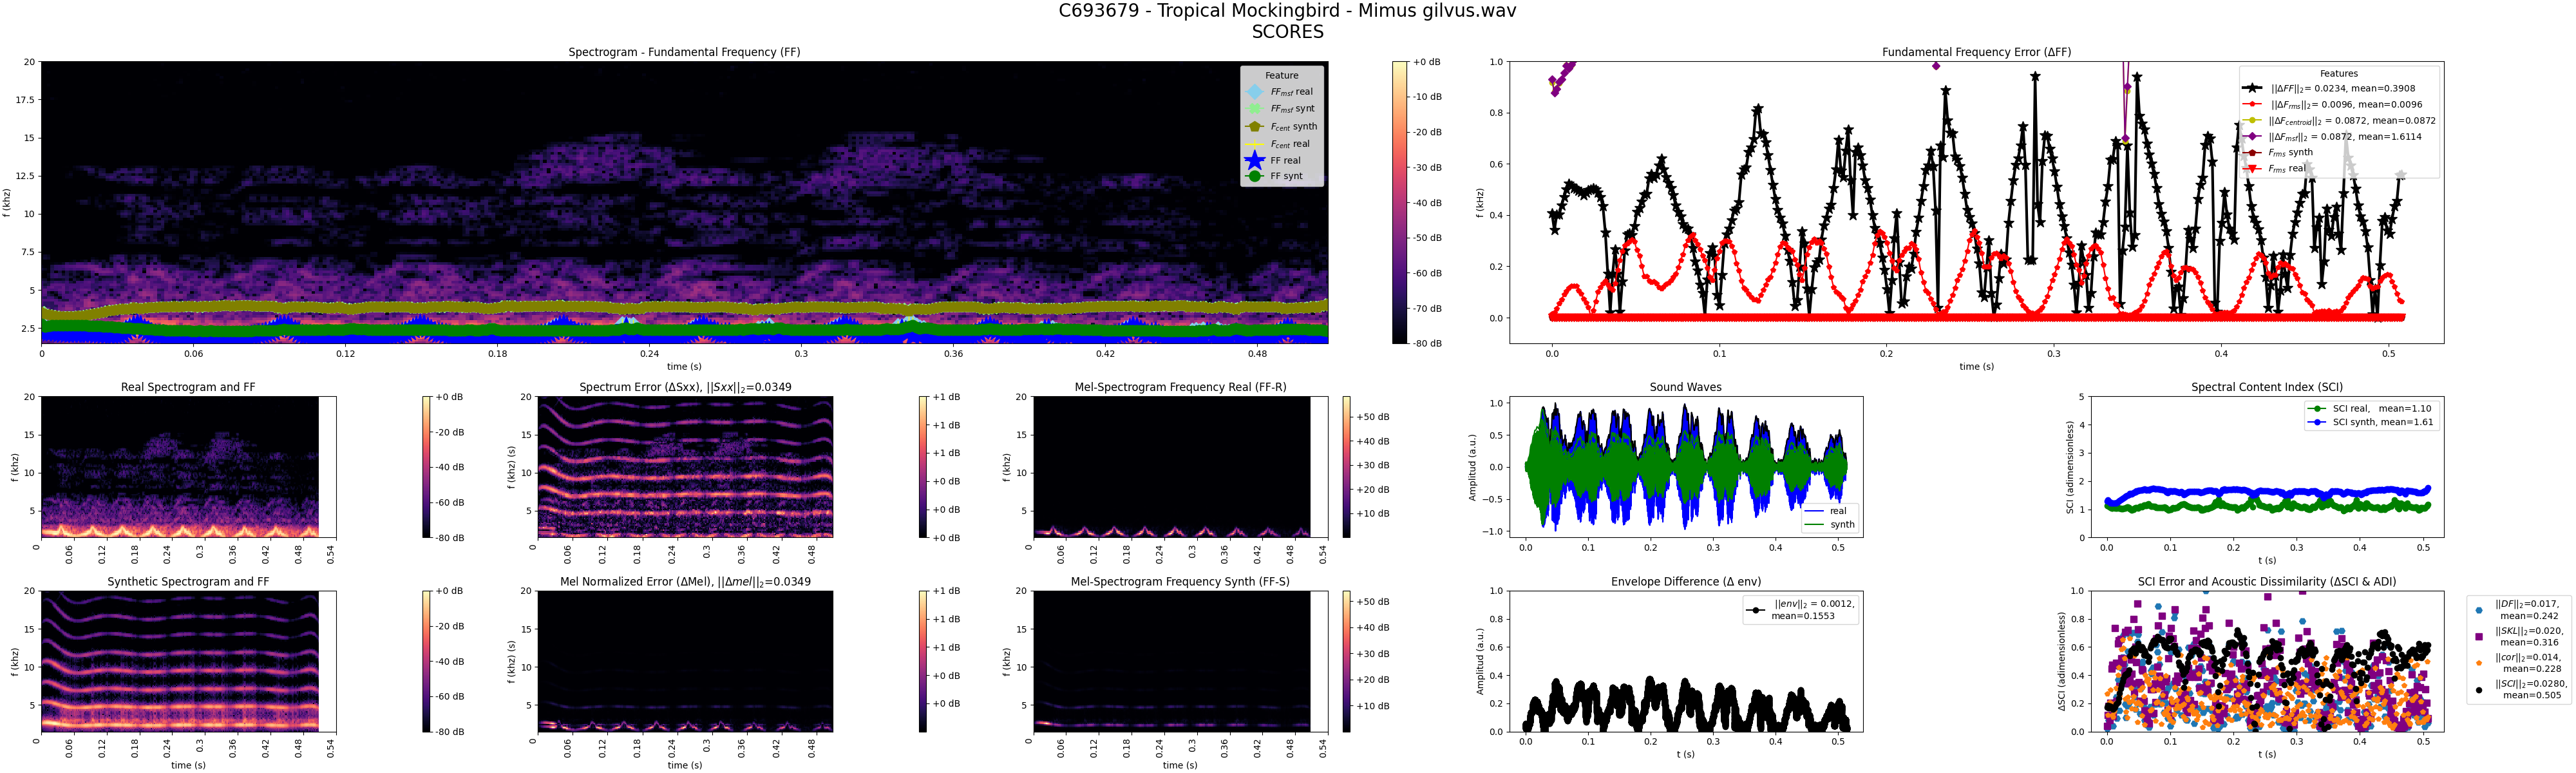
\includegraphics[width=1\linewidth]{Images/ScoresVariables-syllable-C693679 - Tropical Mockingbird - Mimus gilvus.wav-0.png}
    \caption{Simple tropical Mockingbird - Mimus gilvus syllable sample}
    \label{fig:mimus}
    \end{figure}

    
\end{enumerate}

The audios are store on xeno-canto audios collection, you can fin the used audios at the collection \href{https://xeno-canto.org/set/8103}{dissertation}.